\documentclass[aspectratio=169]{beamer}
\usepackage[english]{babel}
\usepackage{amsmath,amsfonts}
\usepackage{multicol}

\usepackage{IEEEtrantools}
\usepackage{multirow}
% beamer setup

%\usecolortheme{dove}

\setbeamertemplate{navigation symbols}{}
\setbeamertemplate{itemize items}[ball]

\usepackage{tikz}
\usetikzlibrary{shapes,arrows}
\usetikzlibrary{positioning}
\tikzstyle{block} = [rectangle, draw, rounded corners]
\tikzstyle{line} = [draw, -latex']

\DeclareMathOperator*{\argmin}{argmin}
\DeclareMathOperator*{\argmax}{argmax}
\DeclareMathOperator{\E}{\mathbb{E}}
\DeclareMathOperator{\I}{\mathbb{I}}

\AtBeginSection[]{
  \begin{frame}[plain]
  \addtocounter{framenumber}{-1}
  \vfill
  \centering
  %\begin{beamercolorbox}[sep=8pt,center,shadow=true,rounded=true]{title}
    %\usebeamerfont{title}
    \Huge{\insertsectionhead\par}%
  %\end{beamercolorbox}
  \vfill
  \end{frame}
}


\newcommand{\backupbegin}{
   \newcounter{framenumberappendix}
   \setcounter{framenumberappendix}{\value{framenumber}}
}
\newcommand{\backupend}{
   \addtocounter{framenumberappendix}{-\value{framenumber}}
   \addtocounter{framenumber}{\value{framenumberappendix}} 
}




\title{The Economics of Shotgun Marriage}
\subtitle{and Household Bargaining}
\author{Egor Kozlov}

\institute{
  Department of Economics\\
  Northwestern University}
  
  
%\setbeamertemplate{footline}[frame number]

\setbeamertemplate{footline}{% 
  \hfill% 
  \usebeamercolor[fg]{page number in head/foot}% 
  \usebeamerfont{page number in head/foot}% 
  \insertframenumber%
  %\,/\,\inserttotalframenumber
  \kern1em\vskip2pt% 
}

 
%  \usepackage{pgf}
%\logo{\pgfputat{\pgfxy(0,0)}{\pgfbox[right,base]{\footnotesize{\insertframenumber\,/\,\inserttotalframenumber}}}}
%\newcommand{\nologo}{\setbeamertemplate{logo}{}}

\let\olditem\item
\renewcommand{\item}{%
\olditem\vspace{\fill}} 

\begin{document}

% REMOVE SLIDE COUNT

\begin{frame}[plain]
\addtocounter{framenumber}{-1}
\date{\scriptsize}
\titlepage
\end{frame}


\begin{frame}
\frametitle{Can Economic Policies Create Successful Marriages?}
\begin{itemize}
\item Reproduction of poverty is a motivation
\item Married two-parent families \ $\genfrac{}{}{0pt}{1}{\Leftarrow \text{ or}}{\Rightarrow \text{  ?}}$ \ desirable outcomes for parents and children%
\item Pro-marriage policies: child support, tax brackets, divorce regulations, etc
\item I propose a measurable dimension of marriage heterogeneity
\end{itemize}
\end{frame}

\begin{frame}

\frametitle{Kids-First Marriages are Closer to The Threshold}
\begin{enumerate}
\item{\textbf{Kids-first couples}} --- child \textit{before or in the year} of marriage
\item{\textbf{Marriage-first couples}} --- child \textit{at the following year or later}
\end{enumerate}
\begin{itemize}
\item Around 1/4 of childbearing marriages are kids-first
\item They have much higher divorce rates, especially among college graduates
\item Natural distinction to study marriage quality
%\item Marginal in economic sense: sensitive to policies 
\end{itemize}
\end{frame}


%
%\begin{frame}
%\frametitle{Questions}
%\begin{itemize}
%\item Drivers of inequality:
%\begin{itemize}
%\item Focusing on unmarried young single mothers omits an important transition
%\item Unplanned pregnancies look different between age and education groups
%\item Divorced parents may be worse than never married
%\end{itemize}
%\item Value of marriage:
%\begin{itemize}
%\item Do pregnancies trigger marriages? If so, why?
%\item If shotgun marriage is risky, why people agree?
%\end{itemize}
%\end{itemize}
%
%\end{frame}


\begin{frame}
\frametitle{Roadmap}
\begin{enumerate}
\item Document the kids-first marriage and its outcomes empirically
\item Use these empirical relations to estimate a model capturing:
\begin{itemize}
\item dynamic bargaining and limited commitment in marriage
\item lifecycle, income and savings
\item fertility and child expenditures
\end{itemize}
\item Use it to correct the data imperfections and answer the questions:
\begin{itemize}
\item Why do the kids-first couples divorce more?
\item Can policies fix the difference or reduce the share?
\item How to promote \emph{good} marriages?
\end{itemize}
\end{enumerate}
\end{frame}

\begin{frame}
\frametitle{Conceptual Framework}
\begin{itemize}
\item Marriages differ in match quality $\psi$ (amount of love)
\item Potential spouses observe their $\psi$ and marry if $\psi > \psi_m$ (\textit{agreement threshold})
\item Match quality evolves, and couple divorces if later $\psi < \psi_d$ (\textit{divorce threshold})
\item Lower $\psi$ implies higher risk of divorce
\item Structural model recovers \textit{distribution} of $\psi$ from the risks of divorce
\end{itemize}
\end{frame}

\begin{frame}
\frametitle{Summary of Results}
\begin{enumerate}
\item Differences in divorce:
\begin{itemize}
\item Kids before marriage lower the agreement threshold, divorce chances increase by 1/3
\item 40--50\% of the kids-first marriages happen \emph{because} of kids
\item Risks of being a single mother and social stigma are the main factors
\end{itemize}
\item Implications for policies:
\begin{itemize}
\item Pushing people to marry more is welfare-decreasing for everyone
\item Making divorce harder has some winners, but people lose on average
\item Child support has limited effects on marriage formation, but increases fertility, stimulates divorce and may hurt children
\end{itemize}
%\item 23\% of women had the first child before their first marriage (kids first)
%\item They are 1.8 times more likely to be divorced than ``marriage first''
%\item College grads: 2.8 times more likely to be divorced
%\begin{itemize}
%\item though smaller kids first share (just 10\%)
%\end{itemize}
%\item My structural model corrects selection and data imperfections
%\item Model results:
%\begin{itemize}
%\item Social stigma + threat of raising the child alone explains most of the difference
%\item Child support $\Rightarrow$ more single mothers, little effect on marriage decisions
%\item Being able to control fertility helps everyone
%\end{itemize}
%\item Model answers: Love $>$ Money. In particular:
%\begin{itemize}
%\item Threat of raising the child alone explains most of the difference
%\item Regulating marriages by policies is both hard and inefficient
%\item Easier control over fertility fixes shotgun marriages and has bigger return
%\end{itemize}
\end{enumerate}
\end{frame}

\begin{frame}
\frametitle{Literature}
\begin{itemize}
\item Empirics on shotgun marriages (demography and sociology):
\begin{itemize}
\item {\small  \color{gray}Gibson-Davis et al (2016), Guzzo (2009),  Nuevo-Chiquero (2014)}
\item I can recover the causal content of these numbers
\end{itemize}
\item Lifecycle models:
\begin{itemize}
\item Dynamic limited commitment for marriage and divorce: {\small  \color{gray}Mazzocco, 2007; Voena, 2015; Low et al., 2018; Shephard, 2019; Blasutto, 2020}
\item Fertility during lifecycle: {\small  \color{gray}Sommer, 2015, Ejrnæs, Jørgensen, 2018}
\item I am the first to estimate a marriage/divorce model with fertility choice
\end{itemize}
\item Policy literature:
\begin{itemize}
\item Empirical: {\small \color{gray}Alessina, Guiliano, 2005;  Tannenbaum, 2020; Rossin-Slater, 2017}
\item Structural: {\small  \color{gray}Forester, 2020; Brown, Flinn, 2011; Kennes, Knowles, 2020}
\item I am the first to consider creation and dissolution of shotgun marriages structurally
\end{itemize}
\end{itemize}
\end{frame}




\section{Empirical Motivation}
\begin{frame}
\frametitle{Sources: ACS 2009--2017 and others}
\begin{itemize}
\item Main exercises and model estimation are done on American Community Survey
%\item Huge sample size and enough information to show many things 
\item Individual marriage and fertility history are observed partially
\begin{itemize}
\item Only the most recent marriage date --- restrict to ``married once'' when matters
\item Pick age $\in [21,40]$ to have good information on fertility
\end{itemize}
\item Smaller datasets with better histories for robustness and extra evidence:
\begin{itemize}
\item Survey of Income and Program Participation (SIPP)
\item More: NSFG and NSFH
\end{itemize}
\end{itemize}
\end{frame}

\begin{frame}[label=kfandmf]
\frametitle{Kids First and Marriage First}
\[\Delta T = \text{Year The First Child Born} - \text{Year The First Marriage Happened}.\]
\begin{itemize}
\item Marriage First \textbf{(MF)}: $\Delta T \in \{1,2,...\}$ (kids at least at the next year)
\item Kids First \textbf{(KF)}: $\Delta T \in \{...,-2,-1,0\}$ (shotgun marriage in a wide sense)
\item Not a full partition%: at 30 only 31\% on the US women have kids and exactly one marriage
\item Most of the comparisons are within this group
\end{itemize}
\hyperlink{extra-restrictions}{\beamerbutton{Extra Restrictions}} 
\end{frame}

\begin{frame}[label=dt_graph]
\frametitle{Kids First Women Are Divorced More Often: Just Look}
\begin{center}
\includegraphics[scale=0.75]{div_5y_by_dt.pdf}
\end{center}
\vspace{-1cm}
\hyperlink{dt_graph_educ}{\beamerbutton{by education}} 
\end{frame}

\begin{frame}[label=dt_more]
\frametitle{Kids First Women Are Divorced More Often: More Evidence}
\begin{itemize}
\item The divorce pattern is present in {all subgroups}
\item The pattern is \textit{sharper} for {college graduates} or those with later births
\item Controlling for many confounders explains no more than a half
\item Step-children drive relatively small part of the result
\end{itemize}
\vspace{1cm}
\begin{tabular}{c c c c}
More results: & \hyperlink{emp-table}{\beamerbutton{subgroups}} & \hyperlink{emp-controls}{\beamerbutton{controls}} & \hyperlink{emp-step}{\beamerbutton{step-children}} 
\end{tabular}

\end{frame}






%\begin{frame}
%\frametitle{Kids First Women Are Divorced More Often: Robustness \& Extra}
%\begin{itemize}
%\item SIPP exercise: smaller sample but full marital history and fertility history
%\begin{itemize}
%\item Similar ratios with larger magnitudes when include remarried people
%\end{itemize}
%\item Duration model: NSFH, historic data from 80s
%\begin{itemize}
%\item Hazard ratio of 1.45, college: 2.23
%\end{itemize}
%\item More details: NSFG, 2015--2017 data
%\begin{itemize}
%\item KF: 30\% true shotgun, 50\% marry after birth, 20\% marry new partner
%\item True shotgun have the highest share of divorced
%\end{itemize}
%\end{itemize}
%\end{frame}
%
%
%\begin{frame}
%\frametitle{Need For The Model}
%\begin{enumerate}
%\item Observables provide limited information. Missing things: relationship quality, potential partners, future divorces
%\item Data are not perfect. Limited histories, unobservable income if out of labor force, step or own children
%\end{enumerate}
%\end{frame}



\section{Model}
\begin{frame}
\frametitle{Summary: Lifecycle, Fertility, Divorce}
\begin{itemize}
\item Lifecycle model with finite horizon
\item People are heterogeneous with respect to age $t$, wages $w$ and savings $a$
\item Couples also differ by relationship quality $\psi$ and spouses' decision power $\theta$
\item Fertility: endogenous decision to have a child (just one) + shocks
\item Limited commitment: decisions are affected by outside options of divorce
\end{itemize}
\end{frame}



\begin{frame}
\frametitle{Modeling Shotgun Marriage}
\begin{center}
\vspace{-0.6cm}
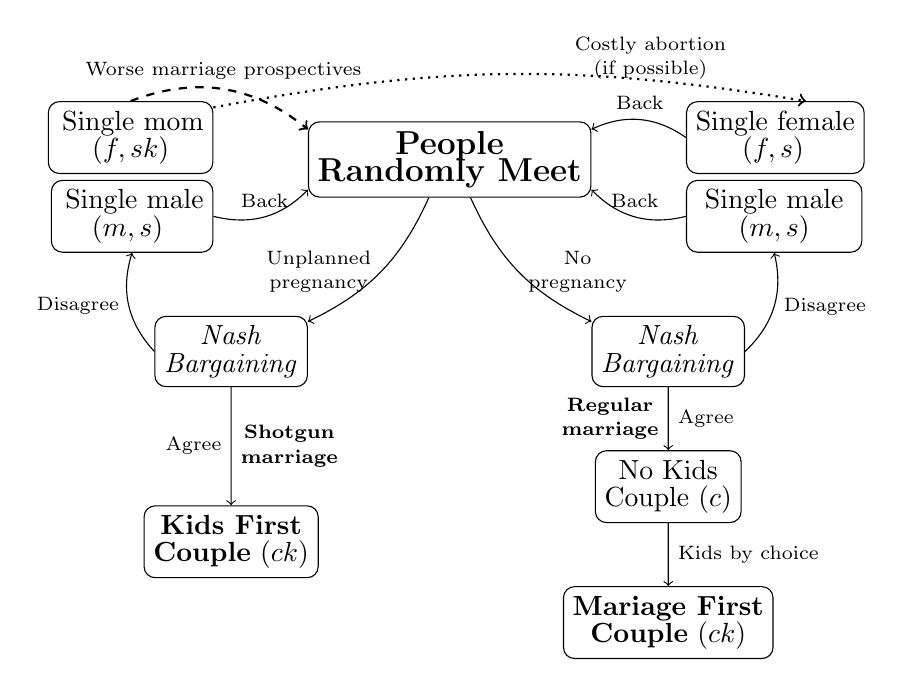
\begin{tikzpicture}[every text node part/.style={align=center}, scale=0.75]
   % Place nodes
   \node [block] (1) {\large \textbf{People}  \\[-0.5ex]  \large  \textbf{Randomly Meet}};
   \node [block, below left = 1.5 cm and 0.0 cm of 1] (2) {\textit{Nash} \\[-0.5ex] \textit{Bargaining}};   
   \node [block, below right = 1.5 cm and 0.0 cm of 1] (3) {\textit{Nash} \\[-0.5ex] \textit{Bargaining}};   

   \node [block, below = 1.5 cm of 2] (5) {\textbf{Kids First} \\[-0.5ex] \textbf{Couple} ($ck$)};
   \node [block, below = 0.8 cm of 3] (7) {No Kids \\[-0.5ex] Couple ($c$)};
   \node [block, below = 0.8 cm of 7] (8) {\textbf{Mariage First} \\[-0.5ex] \textbf{Couple} ($ck$)};
   \draw[->] (1) to [bend left = 20] node [left] {\scriptsize Unplanned \\[-0.75ex] \scriptsize pregnancy} (2);
   \draw[->] (1) to [bend right = 20] node [right] {\scriptsize No \\[-0.75ex] \scriptsize pregnancy} (3);
   \draw[->] (2) to node [left] {\scriptsize Agree} node [right] {\scriptsize \textbf{Shotgun} \\[-0.75ex]  \scriptsize \textbf{marriage}} (5);
   \draw[->] (3) to node [right] {\scriptsize Agree} node [left]  {\scriptsize \textbf{Regular} \\[-0.75ex]  \scriptsize \textbf{marriage}} (7);
   \draw[->] (7) to node [right] {\scriptsize Kids by choice} (8);   
    \node [block, above left   = 0.8 cm and -0.75 cm of 2] (4) {\,Single male \\[-0.5ex] ($m,s$)\,\,};
    \node [block, above left   = 1.8 cm and -0.75 cm of 2] (4-sm) {\,Single mom \\[-0.5ex]  ($f,sk$)};
    %\node [block, left = 0.2 cm of 4-sm] (4-nsm) {\,Single female \\[-0.5ex]  ($f,sk$)};
	\node [block, above right   = 0.8 cm and -0.75 cm of 3] (6) {\,\,Single male\,\,\\[-0.5ex] ($m,s$)};
    \node [block, above right   = 1.8 cm and -0.75 cm of 3] (6-f) {Single female\\[-0.5ex] ($f,s$)\,};   
    \draw[->] (2.180) to [bend left = 30] node [left] {\scriptsize Disagree} (4.270);
    \draw[->,thick,dotted] (4-sm.20) to [bend left = 10] node [above right=-0.2cm and 0.7cm] {\scriptsize Costly abortion \\[-0.75ex] \scriptsize (if possible)} (6-f.50);
    \draw[->] (3.0) to [bend right = 30] node [right] {\scriptsize Disagree} (6.270);
     \draw[->] (6.180) to [bend left = 30] node [above] {\scriptsize Back}  (1.-12);
   \draw[->] (6-f.180) to [bend right = 30] node [above] {\scriptsize Back} (1.12);
   \draw[->,thick,dashed] (4-sm.90) to [bend left = 30] node [above] {\scriptsize Worse marriage prospectives}  (1.168);
   \draw[->] (4.0) to [bend right = 30] node [above] {\scriptsize Back} (1.192);
   
   
\end{tikzpicture}
\end{center}
\end{frame}


\begin{frame}
\frametitle{Value Function: Female, Single}
\framesubtitle{$p^m_t$ --- probability of meeting, $p^p_t$ --- probability of unplanned pregnancy, $m_t$ --- agree to marry}
\begin{align*}
V^{f,s}_t(a,w) = & \max\limits_{c,a'} \Bigg\{ \frac{c^{1-\sigma}}{1-\sigma} + \beta \cdot \E_t  \text{\textbf{Transitions}}_{t+1} \Bigg\}  \\
\text{ \footnotesize (budget constraint): \ } & c + a' = R\cdot a  + w , \\
\text{ \footnotesize (wage evolution): \ } & \log w = z + \text{Trend}_t, \ \ z' = z + \varepsilon^{f}.
\end{align*}
\textbf{Transitions}:
\begin{itemize}
\item \footnotesize No partner met: stay single, $V^{f,s}_{t+1}$, random with probability $1-p^{\text{meet}}_t$
\item \footnotesize Met, no unplanned pregnancy, random with probability $p^{\text{meet}}_t\cdot (1-p^{\text{preg}}_t)$: 
\begin{itemize}
\item \footnotesize Agree to marry: enter couple without a child, $V^{f,c}_{t+1}$
\item\footnotesize  Disagree, stay single: $V^{f,s}_{t+1}$
\end{itemize}
\item \footnotesize Met, no unplanned pregnancy, random with probability $p^{\text{meet}}_t\cdot p^{\text{preg}}_t$: 
\begin{itemize}
\item \footnotesize Agree to marry: enter couple with a child, $V^{f,ck}_{t+1}$
\item \footnotesize Disagree, \textit{pick} $\max\{V^{f,s}_{t+1} - \phi_a, V^{f,sk}_{t+1}\}$ \textit{if abortion is possible ($p^a$), otherwise} $V^{f,sk}_{t+1}$
\end{itemize}
\end{itemize}
\end{frame}


\begin{frame}
\frametitle{Value Function: Couple, No Children}
\framesubtitle{$k_t$ --- give a birth, $d_t$ --- get a divorce, $\tilde{V}$ --- values at divorce}
\begin{align*}
V^{c}_t(a,w_f,w_m,\psi,\theta) = \max\limits_{c_f,c_m,a',k} \Bigg\{ & \theta^f \cdot \frac{c_f^{1-\sigma}}{{1-\sigma}}  + \theta^m \cdot \frac{c_m^{1-\sigma}}{1-\sigma}  + \psi + \beta \cdot \E_t \text{\textbf{Transitions}}_{t+1} \Bigg\}   \\
\text{ \footnotesize (budget constraint, rts): \ } &{\normalsize \left[c_f^{1+\rho} + c_m^{1+\rho}\right]^{\frac1{1+\rho}} + a' = R\cdot a + w_f + w_m}\\
\text{ \footnotesize (match quality evolution): \ } &{\normalsize \psi' = \psi + \varepsilon^{\psi}}\\
\text{ \footnotesize \textbf{(participation constraints)}: \ } &{\normalsize V^{f,c\bullet}_{t+1} (\cdots,\theta') \geq \tilde{V}^{f,s}_{t+1}, \ \ V^{m,c\bullet}_{t+1} (\cdots,\theta') \geq \tilde{V}^{m,s}_{t+1}.}
\end{align*}
\textbf{Transitions}:
\begin{itemize}
\item  \footnotesize Stay together, no birth, choice: $\theta^f \cdot V^{f,c}_{t+1} + \theta^m \cdot V^{m,c}_{t+1}$
\item  \footnotesize Stay together, try to give a birth, choice:
\begin{itemize}
\item  \footnotesize  \textit{If successful} ($p^{\text{birth}}_t$):  $\theta^f\cdot V^{f,ck}_{t+1} + \theta^m\cdot V^{m,ck}_{t+1}$, \textit{otherwise} $\theta^f\cdot V^{f,c}_{t+1} + \theta^m\cdot V^{m,c}_{t+1}$
\end{itemize}
\item  \footnotesize  Divorce, choice: $\theta^f \cdot \tilde V^{f,s}_{t+1} + \theta^m \cdot \tilde V^{m,s}_{t+1}$ (property division + divorce costs inside)
\end{itemize}
\end{frame}


\begin{frame}
\frametitle{Value Function: Couple and Child}
\framesubtitle{$d_t$ --- get a divorce, $\tilde{V}$ --- values at divorce}
\vspace{-1cm}
\begin{align*}
V^{ck}_t(a,w_f,w_m,\psi,\theta) = \max\limits_{c_f,c_m,x,l_f,a'} \Bigg\{ & \theta^f \cdot \frac{c_f^{1-\sigma}}{{1-\sigma}}  + \theta^m \cdot \frac{c_m^{1-\sigma}}{1-\sigma}  + \psi + \\ \text{ \footnotesize (child is a public good): \ }  & \phi + \alpha \cdot \frac{Q^{1-\sigma}}{1-\sigma} +  \beta \cdot \E_t \text{\textbf{Transitions}}_{t+1}  \Bigg\} \\
\text{ \footnotesize (budget constraint): \ } &{\normalsize \left[c_f^{1+\rho} + c_m^{1+\rho}\right]^{\frac1{1+\rho}} + x + a' = R\cdot a + w_f\cdot l_f + w_m}\\
\text{ \footnotesize (child consumption flow): \ } &{\normalsize Q = \left[x^\lambda + \kappa \cdot (1-l_f)^\lambda\right]^{\frac1\lambda}}, \\
\text{ \footnotesize  (subsistence constraint): } & Q\geq \bar{Q} \\
\text{ \footnotesize (female skills $\downarrow$ if not working): \ } &{\normalsize \log w_f = z_f + \text{Trend}_{f,t}, \ \ z'_f = z_f + \varepsilon^f - \delta(l^f)}
\end{align*}
\textbf{Transitions}:
\begin{itemize}
\item  \footnotesize Stay together, choice: $\theta^f \cdot V^{f,ck}_{t+1} + \theta^m \cdot V^{m,ck}_{t+1}$
\item  \footnotesize Divorce, choice: $\theta^f \cdot \tilde V^{f,sk}_{t+1} + \theta^m \cdot \tilde V^{m,s}_{t+1}$ (property division + divorce costs + child support inside)
\end{itemize}
\end{frame}



\begin{frame}
\frametitle{Renegotiation and Divorce}
\framesubtitle{Are generated by the participation constraints}
\begin{itemize}
\item Bargaining weights $\theta$ adjust to satisfy both participation constraints
\[\Delta \theta^i \text{ reflects Lagrange multiplier on $i$'s participation constraint}: V^{i,c\bullet}_{t+1} \geq \tilde{V}^{i,s}_{t+1}\]
\item If no adjustment is possible, the couple divorces
\item Assets are split evenly upon divorce (follows Voena, 2015)
\item Partners have fixed utility costs $\phi_d$ of divorce
\item If couple with a child divorces wife becomes a single mother
\end{itemize}
\end{frame}

\begin{frame}
\frametitle{Child Support}
\framesubtitle{Paid forever, but with a chance to avoid}
\begin{itemize}
\item Imperfect enforcement: probability to be awarded is $p^{\text{award}}$
\begin{itemize}
\item Married couples: 46\%, never married couples: 28\% chances
\end{itemize}
\item If enforced:
\begin{itemize}
\item man loses productivity $z$ so earnings fall by 20\%
\item woman gains productivity $z$ matching this value
\end{itemize}
\item As $z' = z + \varepsilon^z$, all changes are permanent
\end{itemize}
\end{frame}

%\begin{frame}
%\frametitle{Abortions / Birth Control}
%\begin{itemize}
%\item When unplanned pregnancy happens, with probability $p^{\text{access}}$ woman can avoid being single mother
%\item If possible, she pays \emph{fixed utility costs} $u^{a}$ for this
%\item Targets: $\sim40\%$ unplanned pregnancies are aborted + age profile of abortions
%\item Some women \textit{choose} to be single mothers even with abortion access
%\end{itemize}
%\end{frame}

\begin{frame}
\frametitle{Marriage}
\framesubtitle{Introducing Social Stigma}
\begin{itemize}
\item Singles meet singles with random $a$ and $z$ (estimated)
\item Potential couple gets a draw of match quality $\psi$
\item If both partners agree to marry, initial $\theta$ is set by symmetric Nash Bargainig
\item More utility shifters (unexplained things):
\begin{itemize}
\item If unplanned pregnancy happens, partners face {\textbf{social stigma}} $\phi_s$ if refuse to marry
\item If male meets a single mother, he lose $\phi_m$ for having step children
\end{itemize}
\end{itemize}
\begin{center}
{\footnotesize
\begin{tabular}{|l||c|c||c|c||c|}\hline
 & \multicolumn{2}{|c||}{Male gets:} & \multicolumn{2}{|c||}{Female gets:} \\\hline
Situation & Agree & Disagree & Agree & Disagree \\\hline
Regular match & $V^{m,c}_t(\theta)$ & $V^{m,s}_t$ & $V^{f,c}_t(\theta)$ & $V^{f,s}_t$ \\
Unplanned pregnancy & $V^{m,ck}_t(\theta)$ & $V^{m,s}_t - \phi_s$ & $V^{f,ck}_t(\theta)$ & $V^{f,s}_t - \phi_s$ \\
Meeting a single mother & $V^{m,ck}_t(\theta) - \phi_m$ & $V^{m,s}_t$ & $V^{f,ck}_t(\theta)$ & $V^{f,s}_t$ \\\hline
\end{tabular}
}
\end{center}
\end{frame}

\section{Mechanics \& Intuition}
\begin{frame}
\frametitle{Unplanned Pregnancy $\Rightarrow$ Worse Match?}
\framesubtitle{Why people enter knowingly risky marriages?}
\begin{itemize}
\item Women enter the shotgun marriages because:
\begin{itemize}
\item Child costs need to be shared (returns to scale)
\item Finding a new partner is trickier once you have a child
\end{itemize}
\item Men enter the shotgun marriage because:
\begin{itemize}
\item They like their kids and lose access to them otherwise
\end{itemize}
\item Even with a good match, mistimed pregnancy is a risk
\item Scope of these effects depend on exact calibration
\end{itemize}
\end{frame}


\begin{frame}
\frametitle{Unplanned Pregnancy $\Rightarrow$ Women Lose a Lot, Men Gain a Little}
\framesubtitle{Nash Bargaining Surplus: $NBS(\theta) = (V^{f,\text{agree}}(\theta) - V^{f,\text{disagree}})\times(V^{m,\text{agree}}(\theta) - V^{m,\text{disagree}})$}
\begin{center}
\begin{tabular}{c c}
\hspace{-1cm} \includegraphics[scale=0.5]{change_upp.pdf} &
\hspace{-0.5cm}\includegraphics[scale=0.5]{surp_upp.pdf} 
\end{tabular}

\end{center}

\end{frame}

\begin{frame}
\frametitle{...Hence Less Picky Partners + Lower Female Decision Power}
\begin{center}
\begin{tabular}{c c}
\hspace{-1cm} \includegraphics[scale=0.5]{barg_reg_match.pdf} & \includegraphics[scale=0.5]{barg_upp.pdf}
\end{tabular}
\end{center}
\end{frame}


\section{Fit and Results}

\begin{frame}
\frametitle{Too Much Heterogeneity}
\begin{itemize}
\item College and non-college people have very distinct patterns
\item They cannot be summarized well with one-dimensional productivity
\item Therefore I focus on two subsamples:
\begin{itemize}
\item High education: bachelor degree or more
\item Low education: high school or less
\end{itemize}
\item Model fits well for both groups, but high education results are more settled
\end{itemize}
\end{frame}

\begin{frame}
\frametitle{Targets}
\begin{tabular}{l p{0.5\linewidth}}\hline
\multicolumn{1}{l}{Target} & \multicolumn{1}{l}{Informative about} \\\hline
\footnotesize \% with kids 1--10 years after marriage & \footnotesize  Fertility parameters: $\phi$, $\alpha$ \\
\footnotesize \% MF females in population at 23--35 & \footnotesize  $\phi$, $\alpha$ + meeting probabilities \\
\footnotesize \% KF females in population at 23--35 &\footnotesize   meeting + unplanned preg probabilities\\
\footnotesize \% never married with and without kids at 23--35 & \footnotesize  meeting + unplanned preg probabilities + $\phi_r$\\
\footnotesize \% divorced with and without kids at 23--35 & \footnotesize  distribution of $\psi$ + fertility parameters + $\phi_r$ \\
\footnotesize child expenditures share, \% in LF with kids & \footnotesize  household technology: $\kappa$, $\alpha$ and $\bar{Q}$ \\
\footnotesize \% divorced 1--10 years after marriage if KF or MF & \footnotesize  social stigma, $\bar{Q}$ and more ... \\
\footnotesize \% unplanned pregnancies aborted + age profile & \footnotesize  abortion costs and access \\\hline
\end{tabular}
\end{frame}



\begin{frame}
\frametitle{Data}
\framesubtitle{High school in red, college in black}
\begin{center}
\begin{tabular}{c c}
\hspace{-0.5cm} \includegraphics[scale=0.33]{div_kfmf_dc.pdf} & \includegraphics[scale=0.33]{popshares_dc.pdf} \\
\hspace{-0.5cm} \includegraphics[scale=0.33]{evermar_dc.pdf} & \includegraphics[scale=0.33]{everkids_dc.pdf} \\
\end{tabular}
\end{center}
\end{frame}



\begin{frame}
\frametitle{Estimates}
\framesubtitle{Simulated Method of Moments (SMM) with optimization routine from Arnoud et al, 2019; 17 parameters}
\begin{tabular}{l c c c}\hline
& High Education & Low Education & Source \\\hline
\multicolumn{4}{c}{Utility from kids: $\phi + \alpha \cdot \frac{Q^{1-\xi}}{1-\xi}$, \ $Q = [x^{\lambda} + \kappa\cdot(1-l_f)^{\lambda}]^{\frac1{\lambda}}$. $Q\geq \bar{Q}$}\\\hline
$\phi$, $\alpha$, $\kappa$  \footnotesize (utility params) &\footnotesize  $(1.39, 0.36, 0.78)$ &\footnotesize $(1.80,0.45, 1.16)$ & SMM \\
$\bar{Q}$ \footnotesize (subsistence constraint) & 1.7 & 0.70 & SMM\\
\multicolumn{4}{c}{Meeting probability $p^{\text{meet}}$, pregnancy probability $p^{\text{preg}}$: quadratic polynomials}\\\hline
$p^{\text{meet}}$  \footnotesize at (21,30,40) & \footnotesize $(0.11, 0.21, 0.34)$ & \footnotesize  $(0.44, 0.10, 0.65)$ & SMM\\
$p^{\text{preg}}$ \footnotesize  at (21,28,35) & \footnotesize  $(0.01, 0.04, 0.01)$ & \footnotesize  $(0.09, 0.07, -0.05)$ & SMM \\\hline\hline
\multicolumn{4}{c}{Additive utility shifters}\\\hline
$\sigma(\varepsilon^\psi), \sigma(\psi_0)$   \footnotesize (match quality distribution) & $(0.10,0.14)$ & $(0.88,4.8)$ & SMM \\
$\phi_s$ \footnotesize  (social stigma) & 4.21 & 5.31 & SMM\\
$\phi_m$ \footnotesize   (single mom remarriage loss) & 43.3 & 79.6 & SMM \\\hline
$\phi_d$ \footnotesize   (divorce costs) & 5.3 & 1.2 & SMM \\\hline
$(p^{\text{access}}, \phi_a)$ \footnotesize   (abortion parameters) & $(0.22,37.5)$  & $(0.18,5.51) $& SMM \\\hline
\end{tabular}
\end{frame}



\begin{frame}
\frametitle{Things Fit Well --- Part 1}
\framesubtitle{High Education Sample}
\begin{center}

\begin{tabular}{c c}
\hspace{-1cm}\includegraphics[scale=0.5]{evermar.pdf} &\hspace{-0.5cm} \includegraphics[scale=0.5]{popshares.pdf} \\
\end{tabular}
\end{center}
\end{frame}


\begin{frame}
\frametitle{Things Fit Well --- Part 2}
\framesubtitle{High Education Sample}
\begin{center}
\begin{tabular}{c c}
\hspace{-1cm}\includegraphics[scale=0.5]{div_kfmf.pdf}  & \hspace{-0.5cm} \includegraphics[scale=0.5]{everkids.pdf} 
\end{tabular}
\end{center}
\end{frame}

\begin{frame}[label=counterfactuals-abortions]
\frametitle{What Explains The Difference?}
\framesubtitle{Removing Social Stigma (1/4) + Fertility Control (3/4).}
\begin{center}
\begin{tabular}{c c}
\hspace{-1cm}\includegraphics[scale=0.5]{div_kfmf_equalized.pdf}  & \hspace{-0.5cm} \includegraphics[scale=0.5]{relshares_equalized.pdf} 
\end{tabular}
\end{center}
Welfare: men gain $\approx \$35k$, women gain $\approx \$12k$, \hyperlink{welfare-abortions}{\beamerbutton{details}} 
\end{frame}


\begin{frame}[label=counterfactuals-child-support]
\frametitle{Removing Existing Child Support --- Part 1}
\framesubtitle{Less single mothers, less divorces, more abortions}
No child support instead of current (partially enforced 20\%)
\begin{center}
\begin{tabular}{c c}
\hspace{-1cm}\includegraphics[scale=0.5]{div_kfmf_child_support.pdf}  & \hspace{-0.5cm} \includegraphics[scale=0.5]{sm_child_support.pdf} 
\end{tabular}
\end{center}
Just removing the social stigma \hyperlink{counterfactuals-social-stigma}{\beamerbutton{here}} 

Welfare: men gain $\approx \$3k$, women lose $\approx \$1k$ \hyperlink{welfare-child-support}{\beamerbutton{details}} 
\end{frame}

\begin{frame}[label=counterfactuals-child-support]
\frametitle{Removing Existing Child Support --- Part 2}
\framesubtitle{Hardly Affects Marriage in Any Way}
Can you notice the differences?
\begin{center}
\begin{tabular}{c c}
\hspace{-1cm}\includegraphics[scale=0.5]{evermar_cs.pdf}  & \hspace{-0.5cm} \includegraphics[scale=0.5]{popshares_cs.pdf} 
\end{tabular}
\end{center}
\end{frame}



\begin{frame}[label=cf]
\frametitle{More Counterfactuals}
\begin{itemize}
\item No divorce costs \hyperlink{no_divorce_costs}{\beamerbutton{pictures}}
\begin{itemize}
\item More divorces, less kids
\item But less divorces conditional on having kids!
\item Welfare: females lose, males gain, gain on average
\end{itemize}
%\item Removing gender pay gap: same trend + variance for men and women \hyperlink{pay_gap}{\beamerbutton{pictures}} 
\item No unplanned pregnancies at all 
\begin{itemize}
\item Remaining KF (step-child-couples) and MF become very similar
\item Men gain $\sim \$25k$, women gain $\sim \$13k$ 
\item Around 1/10 less divorces
\end{itemize}
\end{itemize}
\end{frame}



\begin{frame}[label=cf]
\frametitle{Conclusions}
\begin{itemize}
\item Model mechanisms can rationalize creation and differences in divorce
\item Child support is welfare-decreasing and does not get people together
\item Controlling fertility helps everyones
\item \textbf{Love $>>$ Money}
%\item Nothing beats the birth control in terms of welfare
%\item Child support does not get people together and creates more single mothers
%\item Empirically, more control over fertility $\Rightarrow$ less KF, lower differences in performance
\end{itemize}
\end{frame}





\backupbegin



%\begin{frame}[label=remarriage_penalty]
%\frametitle{Removing Remarriage Penalty For Single Mothers}
%\framesubtitle{Divorced in 10 years if KF: 13.5\% $\to$ 12.4\%. Divorced in cross-section if KF: 9.3\% $\to$ 8.9\% + More Kids}
%\begin{center}
%\begin{tabular}{c c}
%\hspace{-1cm} \includegraphics[scale=0.5]{div_kfmf_no_remar.pdf}  &  \includegraphics[scale=0.5]{ever_kids_no_remar.pdf} 
%\end{tabular}
%\end{center}
%\hyperlink{cf}{\beamerbutton{back}} 
%\end{frame}



\begin{frame}[label=no_divorce_costs]
\frametitle{No Divorce Costs}
\framesubtitle{Less kids, more shotgun marriages (relatively), less divorces if have kids}
\begin{center}
\begin{tabular}{c c}
\hspace{-1cm} \includegraphics[scale=0.5]{popshares_nodivcosts.pdf}  &  \includegraphics[scale=0.5]{div_kfmf_nodivcosts.pdf} 
\end{tabular}
\end{center}
\hyperlink{cf}{\beamerbutton{back}} 
\end{frame}

\begin{frame}[label=pay_gap]
\frametitle{Removing Pay Gap}
\framesubtitle{Divorced in 10 years if KF: 13.5\% $\to$ 12.6\%. Divorced in cross-section if KF: 9.3\% $\to$ 8.8\% + Fewer Kids}
\begin{center}
\begin{tabular}{c c}
\hspace{-1cm} \includegraphics[scale=0.5]{eq_pay.pdf}  &  \includegraphics[scale=0.5]{everkids_eq_pay.pdf} 
\end{tabular}
\end{center}
\hyperlink{cf}{\beamerbutton{back}} 
\end{frame}




\begin{frame}[plain,label=extra-restrictions]
\frametitle{Extra Restrictions}
\begin{itemize}
\item I do not classify as KF or MF people with $\Delta T < -5$ or $\Delta T > 5$
\item I exclude small share of people with marital statuses ``separated'', ``widowed'' and ``spouse absent''
\item This does not affect the results much but helps to ensure consistency
\end{itemize}
\hyperlink{kfandmf}{\beamerbutton{back to KF and MF}} 
\end{frame}



\begin{frame}[plain,label=emp-table]
\frametitle{Kids First Women Are Divorced More Often: Quantification}
\framesubtitle{ACS 2009--2017, Women 21--40, married once}
\begin{center}
\begin{tabular}{l r r r r }
\hline
& \multicolumn{2}{c}{share of divorced if ... }&  \\
&  marriage-first & kids-first & (share of kids-first) &  \\\hline
\multicolumn{5}{l}{\textbf{All sample}} \\\hline
\textit{Cross-sectional share of divorced} &  9.9 & 18.1 & (26.1) \\
\textit{Divorced 5 years after marriage} &  5.1 & 14.3  & (24.6) \\
\textit{Divorced 10 years after marriage} & 10.4 & 22.8 & (24.4) \\\hline
\multicolumn{5}{l}{\textbf{Cross-sectional share of divorced for subsamples}} \\\hline
\textit{High school only} &  12.8 & 17.3 & (37.0) \\
\textit{Some college} & 14.3 & 21.0 & (31.3) \\
\textit{College or more} &   5.3 & 14.8 & (11.9) \\\hline
\textit{First birth before 25} & 15.5 & 19.9 & (41.8) \\
\textit{First birth at 25 or later} &  6.2 & 10.9 & (10.7)  \\\hline
\end{tabular}
\end{center}
\hyperlink{dt_more}{\beamerbutton{back}} 
\end{frame}

\begin{frame}[plain,label=emp-controls]
\frametitle{Kids First Women Are Divorced More Often: Controls}
\begin{center}
%\vspace{-0.5cm}
\begin{tabular}{l r r r }
\multicolumn{4}{c}{\textit{Regression equation:} $\text{Divorced}_i = \Delta \cdot \text{kids-first}_i + \text{Controls}_i + \varepsilon_i$} \\\hline
\hline
& \multicolumn{2}{c}{Estimates}  \\
& Difference ($\Delta$) & (standard error)  \\\hline
\multicolumn{4}{l}{\textbf{All sample, regression}} \\\hline
\textit{No controls (raw difference) }& 8.2 & (0.1)  \\
\textit{Demographic controls }& 5.7 & (0.1)  \\
\textit{Duration controls} &  5.8 & (0.2)  \\
\textit{Demographic + duration} &  4.8 & (0.2)  \\
\textit{Demographic + duration + income} & 4.1 & (0.3)  \\\hline
\multicolumn{4}{l}{\textbf{All sample, propensity score matching}} \\\hline
\textit{Demographic controls} & 5.0 & (0.3)  \\
\textit{Demographic controls + income} & 4.9 & (0.2)  \\\hline
\multicolumn{4}{p{0.825\linewidth}}{\footnotesize \textit{Controls:} demographics: FE for age $\times$ education, race, state, survey year. Duration: FE for age $\times$ age of the first marriage and age $\times$ age of the first birth.  Income: 3rd degree polynomial of log gross income (if observed).}\\\hline\hline
\end{tabular}
\end{center}
\vspace{-0.5cm}
\hyperlink{dt_more}{\beamerbutton{back}} 
\end{frame}


\begin{frame}[plain,label=emp-step]
\frametitle{Kids First Women Are Divorced More Often: Extra Evidence from SIPP}
\begin{center}
\begin{tabular}{l r r }
\hline
\multicolumn{3}{l}{\textbf{Including remarried people...}} \\\hline
& \multicolumn{2}{c}{share of divorced if ... }  \\
&  marriage-first & kids-first   \\\hline
\textit{Ever divorced} & 34.4 & 48.0  \\
\textit{Divorced if married once} &  12.4 & 19.3 \\
\textit{Remarried} &  22.0 & 28.7 \\\hline
\hline
\multicolumn{3}{l}{\textbf{Separating step and own children (2+ kids only)}} \\\hline
& share in sample & share of divorced   \\\hline
{Marriage-first} & 72.1 & 10.5 \\
{Kids-first-own} &  16.4 & 14.6 \\
{Kids-first-other} &  11.4 & 27.2 \\\hline
\multicolumn{3}{p{0.7\linewidth}}{\footnotesize \textit{Notes.} SIPP data, the cross-section of Wave 1, 2014, women 21+. Numbers are percents.}\\\hline\hline
\end{tabular}
\end{center}
\hyperlink{dt_more}{\beamerbutton{back}} 
\end{frame}


\begin{frame}[plain,label=dt_graph_educ]
\frametitle{Kids First Women Are Divorced More Often: By Education}

\begin{tabular}{c c}
\hspace{-0.5cm}\includegraphics[scale=0.5]{div_5y_by_dt_col.pdf} & \hspace{0.5cm}\includegraphics[scale=0.5]{div_5y_by_dt_hs.pdf}
\end{tabular}
\hyperlink{dt_graph}{\beamerbutton{back to the main graph}} 
\end{frame}



\begin{frame}[label=counterfactuals-social-stigma]
\frametitle{Removing Social Stigma}
\framesubtitle{Less single mothers, less divorces, more abortions}
No child support instead of current (partially enforced 20\%)
\begin{center}
\begin{tabular}{c c}
\hspace{-1cm}\includegraphics[scale=0.5]{div_kfmf_ss.pdf}  & \hspace{-0.5cm} \includegraphics[scale=0.5]{sm_among_mothers_ss.pdf} 
\end{tabular}
\end{center}
\hyperlink{counterfactuals-child-support}{\beamerbutton{back}} 
\end{frame}


\begin{frame}[label=welfare-abortions]
\frametitle{What Explains The Difference? Welfare Implications}
\framesubtitle{Removing Social Stigma (1/4) + Fertility Control (3/4)}
\begin{center}
\begin{tabular}{c c}
\hspace{-1cm}\includegraphics[scale=0.5]{welfare_female_equalized.pdf}  & \hspace{-0.5cm} \includegraphics[scale=0.5]{welfare_male_equalized.pdf} 
\end{tabular}
\end{center}
\hyperlink{counterfactuals-abortions}{\beamerbutton{back}} \hyperlink{welfare-methodology}{\beamerbutton{methodology}} 
\end{frame}

\begin{frame}[label=welfare-child-support]
\frametitle{Child Support Removal}
\framesubtitle{More abortions but not much changes...}
\begin{center}
\begin{tabular}{c c}
\hspace{-1cm}\includegraphics[scale=0.5]{welfare_female_child_support.pdf}  & \hspace{-0.5cm} \includegraphics[scale=0.5]{welfare_male_child_support.pdf} 
\end{tabular}
\end{center}
\hyperlink{counterfactuals-child-support}{\beamerbutton{back}} \hyperlink{welfare-methodology}{\beamerbutton{methodology}} 
\end{frame}

\begin{frame}[label=welfare-methodology]
\frametitle{Definitions}
\framesubtitle{Equivalent Variation (EV) Style}
Value of any policy change can be computed in terms of equivalent amount of assets.

If the change is preferred:
\[EV = a^*_t(w) \text{ such that } V_{t}^{f,s,\text{no change}}(a=a^*,w) = V_{t}^{f,s,\text{with change}}(a=0,w)\]
Otherwise:
\[EV = -a^*_t(w) \text{ such that } V_{t}^{f,s,\text{with change}}(a=a^*,w) = V_{t}^{f,s,\text{no change}}(a=0,w)\]

Analogously for $m$, a bit trickier for couples.

\hyperlink{welfare-abortions}{\beamerbutton{back to abortions}} \hyperlink{welfare-child-support}{\beamerbutton{back to child support}}


\end{frame}

\backupend
\end{document}


